\documentclass{article}
\bibliographystyle{apalike}
% Language setting
% Replace `english' with e.g. `spanish' to change the document language
\usepackage[english]{babel}

% Set page size and margins
% Replace `letterpaper' with `a4paper' for UK/EU standard size
\usepackage[letterpaper,top=2cm,bottom=2cm,left=3cm,right=3cm,marginparwidth=1.75cm]{geometry}

% Useful packages
\usepackage{amsmath}
\usepackage{graphicx}
\usepackage[colorlinks=true, allcolors=blue]{hyperref}

\usepackage{float}
\usepackage{subcaption}

\title{Human Tracking Using The Extended Kalman Filter}
\author{Abolghasem Esmaeily}
\date{February 2024}

\begin{document}
\maketitle


\begin{abstract}

\end{abstract}
Human tracking in video surveillance has become increasingly crucial for enhancing security and safety in various settings. This project aims to develop an advanced human tracking system by leveraging the YOLO (You Only Look Once) model for object detection and the Extended Kalman Filter (EKF) for dynamic tracking of individuals across video frames. By using the OpenCV and PyTorch libraries, our methodology demonstrates significant improvements in detection and tracking accuracy under varying conditions. Preliminary results indicate the system's ability to track individuals, even in scenarios with obstacles. The integration of YOLO with EKF presents a robust solution that could be applied to real-world surveillance and monitoring tasks. This project has the potential to combine deep learning models with filtering techniques to advance the field of computer vision.\\

Keywords: human tracking, YOLO model, Extended Kalman Filter, object detection, video surveillance.

\newpage
\section{Introduction:}

As society grows, the need for security and order becomes greater to avoid crimes. One solution is video surveillance, which leads to an increase in the number of cameras. Due to a lack of human resources, this could be very difficult. That is why a new computer vision algorithm is needed to perform this test. One important component in the field of computer vision is human tracking, which focuses on the identification and continuous observation of individuals across the sequence of images in video frames. This technology helps in a variety of applications, from surveillance and security systems to interactive systems and reality. The objective is to detect human subjects in dynamic environments and track their movements and behaviors over time, which requires algorithms to handle real-world variability and unpredictability. It involves two key stages: detection and tracking. 

\subsection{Object Detection in image/video} 
Object detection is a crucial process in computer vision, aimed at identifying and localizing objects within images or videos. This process involves not only the classification of objects and determining what they are, but also delineating their precise boundaries within the images, typically represented as bounding boxes. Advanced object detection algorithms are designed to operate effectively under a wide range of conditions, accurately recognizing objects despite challenges such as variations in size, orientation, lighting, and even partial occlusion. These capabilities are essential for systems that require robust performance in diverse and dynamically changing environments \cite{visoai2021object}. One of the most popular techniques to satisfy those requirements is You Only Look Once (YOLO).


\subsection{Tracking Objects Across Frames}Detection alone is not sufficient to be sure that detections from frame to frame belong to the same individual. Bridging this gap is the domain of object tracking, which extends the concept of object detection by maintaining the identification and location of objects across successive frames, assigning a unique ID to each detected object. This method involves predicting the movement of each object from one frame to the next, considering factors such as speed, direction, and changes in appearance over time \cite{learnopencvYOLOv8Tracking}. This is where the Extended Kalman Filter (EKF) comes in.

\subsection{Extended Kalman Filter}The Extended Kalman Filter (EKF) is an advanced algorithm designed for estimating the states of a nonlinear dynamic system based on a series of noisy measurements. In human tracking applications, the EKF is utilized to predict the future states of subjects from observed movements. Integrating EKF with object detection models like YOLO can significantly improve tracking accuracy, particularly in scenarios characterized by complex movement patterns. The EKF refines its estimates over time, enhancing the accuracy of predictions with each new observation.\\

\section{Project Goals}
The primary goal of this project is to develop a robust human tracking system that can predict the trajectories of individuals in video footage. Our system integrates the YOLO object detection algorithm with the EKF to improve tracking accuracy and performance. Specific objectives include:
\subsection{Integration of EKF with YOLO}
By combining the EKF algorithm and YOLO-based object detection, we create a system that combines YOLO´s speed and accuracy in object detection with EKF´s precision in prediction and estimating the state of moving objects.
\subsection{Real-time Tracking}
To achieve real-time tracking performance, we need to be sure that the system can handle it effectively in dynamic environments where accurate tracking of human movements is critical. Thus, we are testing the system across diverse scenarios. 

\section{Project Limitations}
Due to computational constraints and the complexity of real-time processing, the system can handle tracking a maximum of two individuals simultaneously.

\subsection{Tracking Capabilities Behind Obstacles}
The system´s ability to track individuals behind obstacles is constrained by the limitations of visual line-of-sight and occlusion. While EKF can predict movements during a short period of occlusion based on previous trajectories, complex environments with multiple obstructions will reduce tracking accuracy.\\


\section{Meethodology:}
\subsection{Implementation of the Human Tracking Algorithm}
The primary goal was to develop an algorithm capable of tracking humans across video sequences. A critical prerequisite for tracking was the ability to detect humans within these sequences correctly. To achieve this, we employed the renowned object detection model known as "YOLO" (You Only Look Once) \cite{learnopencvYOLOv8Tracking}. This model attempts to identify human figures within an image by generating bounding boxes around each detected figure.

As YOLO operates on static images, our approach was to decompose the video into individual frames. This conversion makes it possible to apply the Yolo model to each frame, resulting in an image of humans distinctly marked by bounding boxes. With this setup, tracking human movements across frames became feasible.

\subsection{Tracking Strategy}
Our algorithm's core strategy for tracking was to use the previously identified positions of humans to forecast their future locations in upcoming frames. By employing this predictive technique, it became possible to correlate the detected humans in a new frame with their corresponding predictions from earlier frames. The uncertainty in predicting future positions required a robust solution to be able to handle non-linear dynamics. Thus, we chose the Extended Kalman Filter (EKF) for its efficacy in predicting the state of non-linear systems based on historical data.
The subsequent step is aligning the predicted positions with the actual detections in the current frame. This alignment was achieved by matching each prediction with the nearest bounding box. The human within a bounding box that closely matched a prediction was considered to be the same individual from the preceding frame. This methodology was our approach to human tracking. 


\subsection{Objectc Detection Methodology}
As detailed earlier, our approach to human detection videos required the segmentation of the videos into individual frames, making them suitable for analysis by the YOLO algorithm. The conversion of videos into a series of frames is provided by the OpenCV library \cite{opencv}, a Python-based toolkit designed for processing images and video footage in computer vision. Additionally, the PyTorch framework was utilized to integrate and deploy the YOLO model within our project \cite{pytorch}.

For object detection, we employed the YOLOv5 model, which has been trained on the COCO dataset—a comprehensive image dataset created by Microsoft \cite{lin2014microsoft}.
This model is able to identify a wide array of objects, totaling 80 different categories, with humans being one of them. To ensure the focus remained solely on human figures, we implemented a filtering mechanism. This mechanism screened the YOLO model's output, discarding any bounding box that did not correspond to the "person" category. In order to determine the effectiveness of our human tracking solution, we developed a visualization technique. This technique involved the bounding boxes generated by the YOLO model onto the original frames. Each bounding box was color-coded to represent a unique individual, thereby facilitating an intuitive understanding of the tracking accuracy \cite{ourvisualization2023}.

\subsection{Position Prediction}
The Extended Kalman Filter (EKF) was used to forecast the future locations of detected humans. Utilizing previous states and measurements, the ELF estimates the positions of humans surrounded by bounding boxes. Rather than calculating the dimensions of these bounding boxes—which vary across frames—we focused on the central point of each bounding box as the primary state for prediction.
Positions within a 2D plane are determined by \(x, y\) coordinates, necessitating that the EKF estimate both coordinates' positions. It does so by calculating the states of \(x\) and \(y\) based on the estimated velocity and acceleration, which are derived from the displacement and velocity changes between frames, respectively.
The state vector formulation is represented as:
\begin{equation}    \overline{x} = \begin{bmatrix} x & \dot{x} & \ddot{x} & y & \dot{y} & \ddot{y} \end{bmatrix}    \label{StateVec}\end{equation}
The transition matrix is defined:
\begin{equation}    \Sigma = \begin{bmatrix}1 & \Delta{t} & \frac{{\Delta{t}}^2}{2} & 0 & 0 & 0\\0 & 1 & \Delta{t} & 0 & 0 & 0\\0 & 0 & 1 & 0 & 0 & 0\\0 & 0 & 0 & 1 & \Delta{t} & \frac{{\Delta{t}}^2}{2}\\0 & 0 & 0 & 0 & 1 & \Delta{t}\\0 & 0 & 0 & 0 & 0 & 1\\\end{bmatrix}    \label{TransMat}\end{equation}
This linearization accounts for the time derivatives of position and velocity. The measurement matrix, which reflects the observed central positions of bounding boxes and their uncertainties, is defined as:
\begin{equation}    R = \begin{bmatrix} {{\sigma}_x}^2 & 0 \\ 0 & {{\sigma}_y}^2 \end{bmatrix}    \label{MeasurementMat}\end{equation}
Given the variability in bounding box dimensions, the state covariance matrix \(\textbf{P}\) was introduced to model this uncertainty:
\begin{equation}    P = \begin{bmatrix} \textbf{Cov} & 0 & 0 & 0 & 0 & 0\\ 0 & \textbf{Cov} & 0 & 0 & 0 & 0\\ 0 & 0 & \textbf{Cov} & 0 & 0 & 0\\ 0 & 0 & 0 & \textbf{Cov} & 0 & 0\\ 0 & 0 & 0 & 0 & \textbf{Cov} & 0\\ 0 & 0 & 0 & 0 & 0 & \textbf{Cov} \end{bmatrix}    \label{StateCovMat}\end{equation}
The process noise, reflecting uncertainties in position due to velocity and acceleration, was modeled as:
\begin{equation}    Q = {{\sigma}_\alpha}^2 \begin{bmatrix} \frac{{\Delta{t}}^4}{4} & \frac{{\Delta{t}}^3}{2} & \frac{{\Delta{t}}^2}{2} & 0 & 0 & 0\\ \frac{{\Delta{t}}^3}{2} & {\Delta{t}}^2 & \Delta{t} & 0 & 0 & 0\\ \frac{{\Delta{t}}^2}{2} & \Delta{t} & 1 & 0 & 0 & 0\\ 0 & 0 & 0 & \frac{{\Delta{t}}^4}{4} & \frac{{\Delta{t}}^3}{2} & \frac{{\Delta{t}}^2}{2}\\ 0 & 0 & 0 & \frac{{\Delta{t}}^3}{2} & {\Delta{t}}^2 & \Delta{t}\\ 0 & 0 & 0 & \frac{{\Delta{t}}^2}{2} & \Delta{t} & 1 \end{bmatrix}    \label{ProcNoisetMat}\end{equation}
For every detected individual, a distinct EKF instance is initialized to track the progression of their bounding box. In cases of occlusion, the EKF relies on the last known velocity and acceleration to predict future positions until a new measurement can be obtained, facilitating a return to convergence upon the individual's reappearance.


\subsection{Tracking Process}
Upon generating predicted positions for each bounding box via the Extended Kalman Filter (EKF), the next challenge is accurately maintaining the identity of each detected human across frames. This process requires matching each predicted position with the correct bounding box in the subsequent frame.

To facilitate this matching process, our algorithm uses a distance-based classification method. Specifically, it computes the Euclidean distance between each EKF prediction and the center points of all detected bounding boxes within the same frame. The bounding box with the minimum distance to a given prediction is then associated with that prediction. Consequently, this approach implies that the individual represented by a particular bounding box is identified as the same across frames, based on the proximity of the center points to the predicted positions.

This method resolves the identity and ensures that each human is tracked accurately over time, despite potential movements or changes in the visual field.



\subsection{Evaluation Methodology}
To ascertain the precision of our tracking algorithm on a specific video, we implemented a method that calculates the Euclidean distance between each predicted position and its corresponding assigned bounding box. This measurement process remains for the duration that the tracked individual remains visible within the video frames. It's important to note that during periods of occlusion, where the tracked individual is not visible, this error calculation is suspended to avoid inaccuracies in the evaluation.

After the video analysis, these calculated errors are visualized through a plot that correlates the error magnitude with the frame number. This visualization specifically highlights frames where bounding boxes are detectable, aligning with our methodology of excluding error calculations in frames marred by occlusion. This approach provides a clear, frame-by-frame illustration of the algorithm's tracking accuracy over time.

\section{Results Analysis}
This section presents and examines the outcomes of our object-tracking. We evaluated the performance of our algorithm through a series of tests involving video footage that includes diverse scenarios: a single individual walking behind a whiteboard, two individuals walking sequentially behind a whiteboard, and two individuals crossing paths. These test videos were recorded within the U-Building at the KTH Royal Institute of Technology, providing a consistent setting for our experiments.

To optimize tracking performance, we fine-tuned the process noise parameters, specifically setting the standard deviation values for both the \(x\) and \(y\) coordinates to 0.05 (\(R\), with \(std\_x = 0.05\) and \(std\_y = 0.05\)). This adjustment was critical in achieving the most accurate tracking results under the tested conditions.

\subsection{Video Analysis Results}
\subsubsection{Scenario: Single Individual Moving Behind a Whiteboard}
In this test scenario, we fine-tuned the process noise parameters to \(std\_x = 0.000025\) and \(std\_y = 0.0001\), aiming to evaluate the tracking system's proficiency in handling partial occlusions, such as a person walking behind a whiteboard. The chosen small values for the standard deviations of the process noise reflect relatively smooth and predictable motion trajectories. As a result, the system is generally capable of maintaining a consistent prediction of the path, by to the minimized process noise.

During the video assessment, as the individual passes behind a whiteboard, the tracking marker—visualized as a dot—largely follows the anticipated direction of movement. The tracking precision is compromised during moments of occlusion; this is particularly noticeable when the individual comes from behind the whiteboard. The apparent deviation between the predicted trajectory and the actual location of the person upon reentry into the visible area highlights a critical challenge for the tracking system: preserving positional accuracy in the face of obstructions.

\begin{figure}[H]
\centering
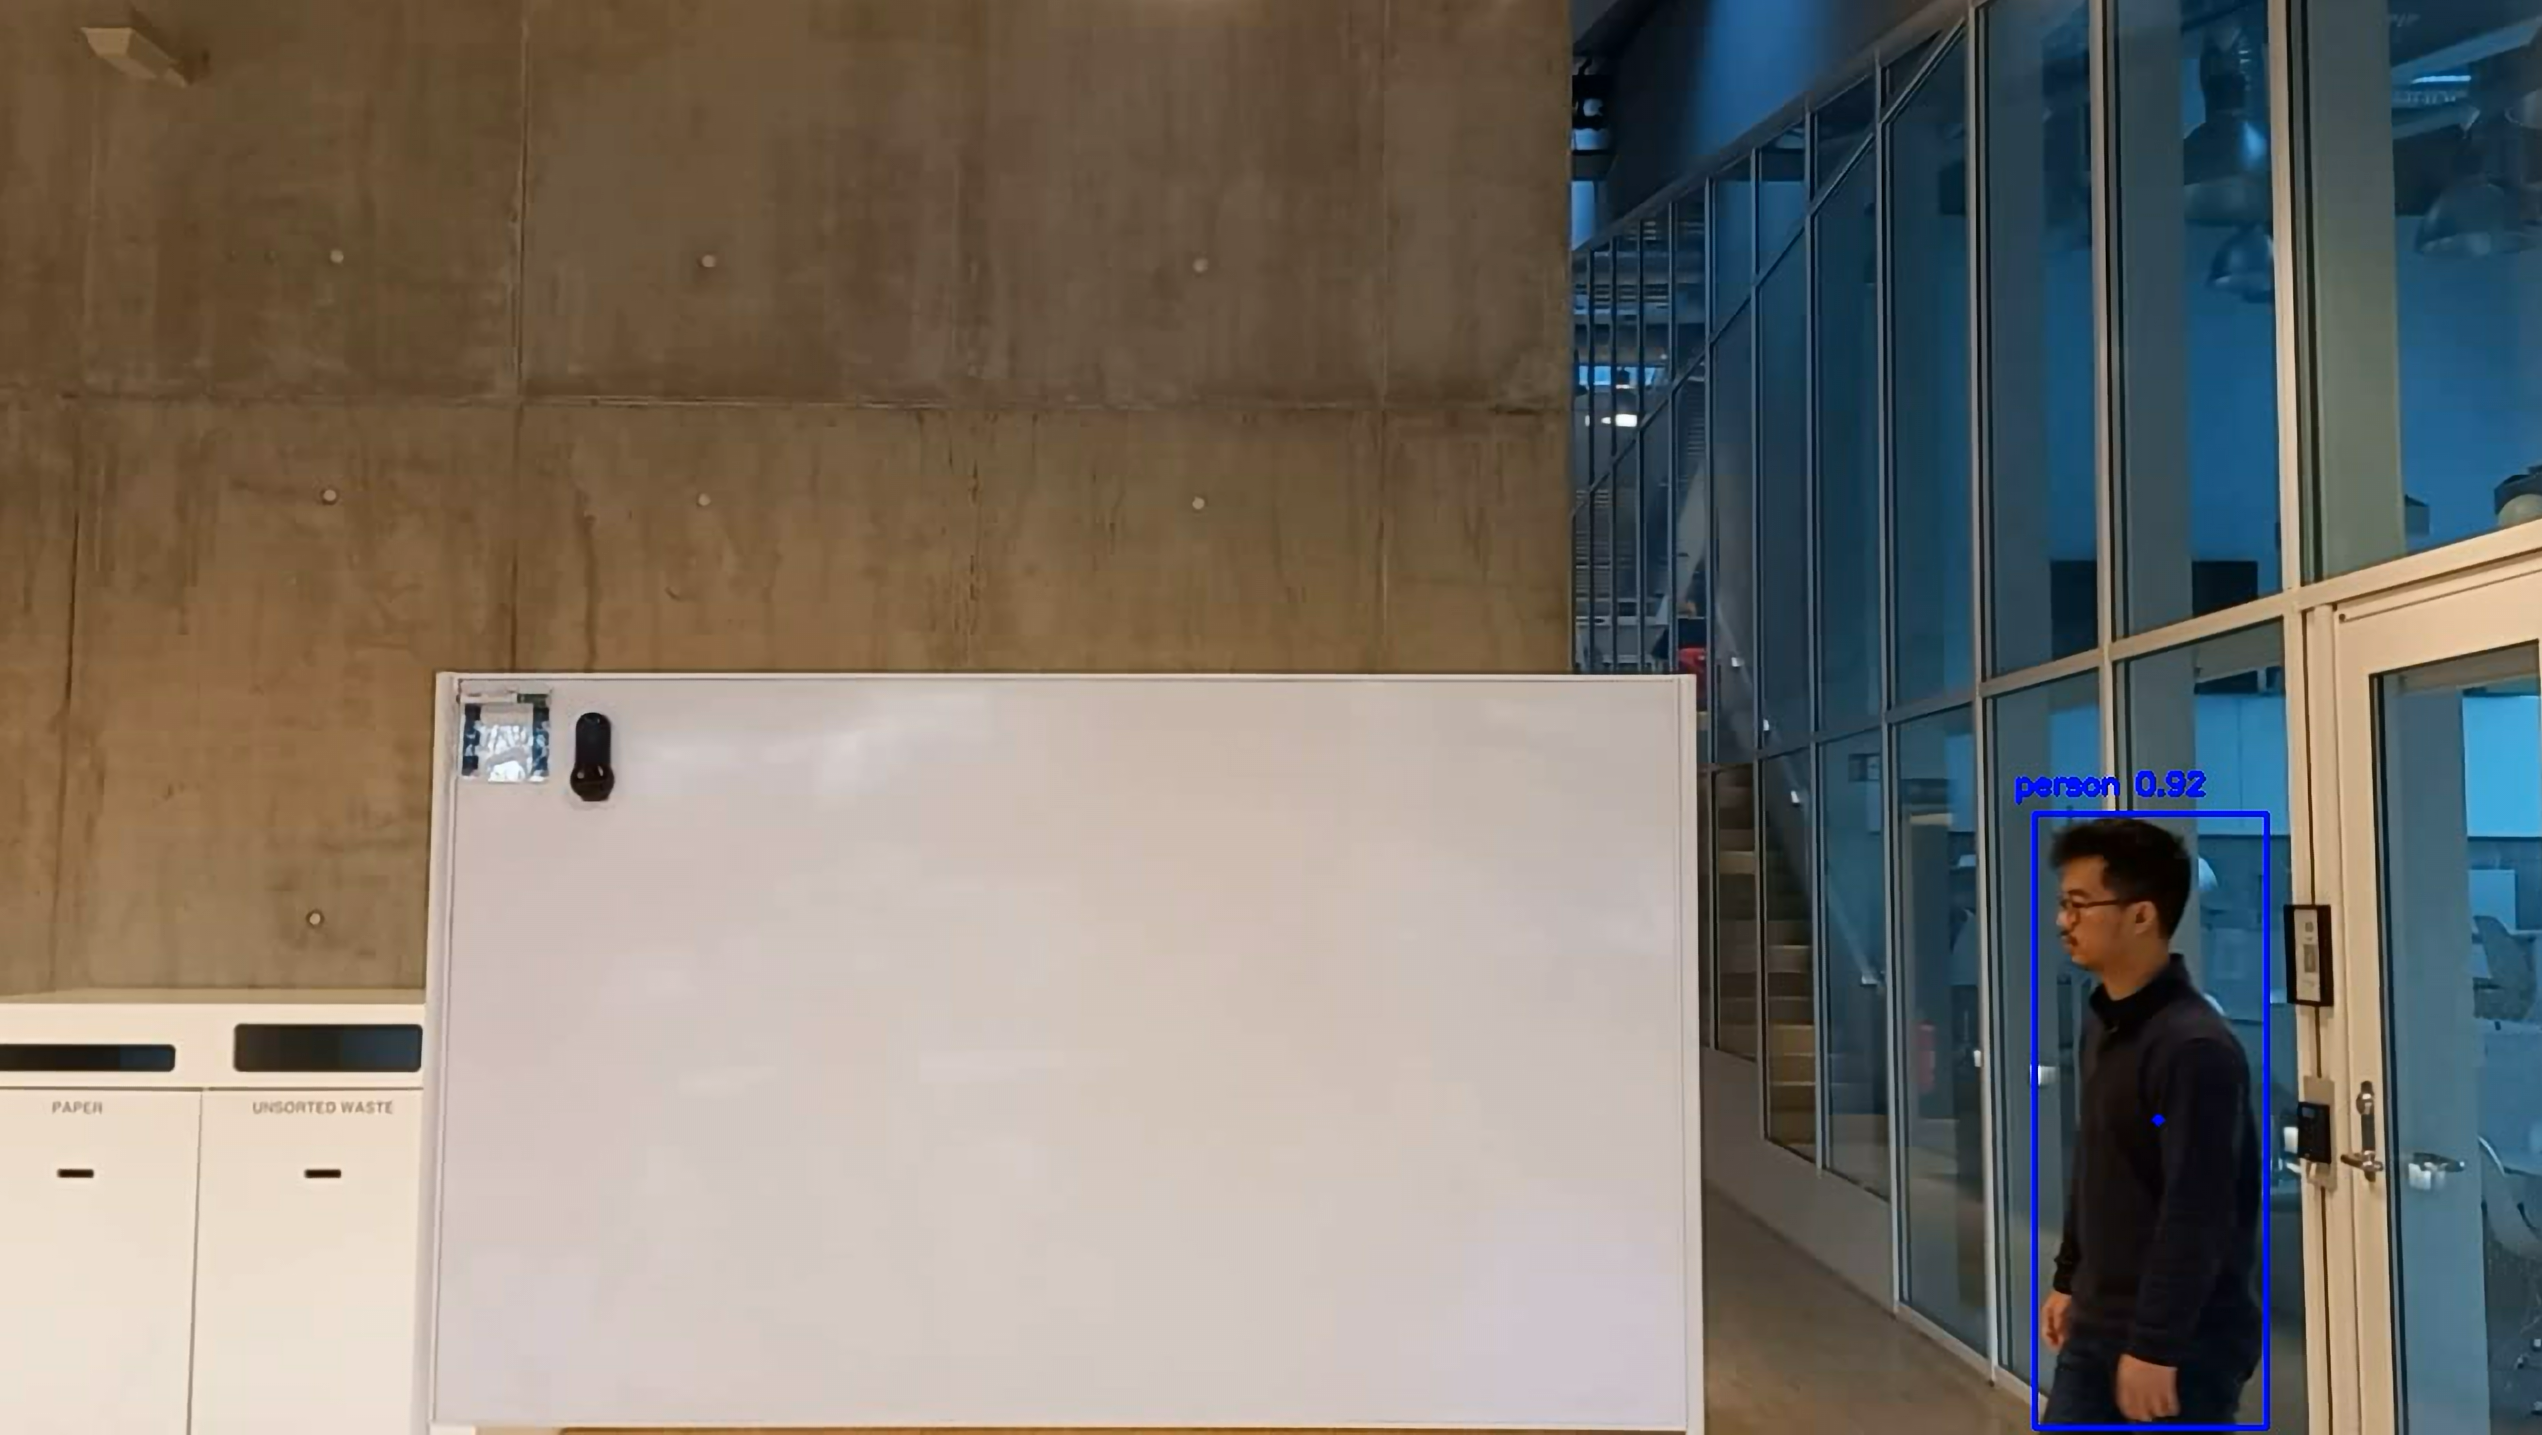
\includegraphics[width=0.5\linewidth]{one people.png}
\caption{One Person When Passing Behind a Whiteboard}
\label{fig:one human}
\end{figure}

\subsubsection{Two Humans Passing Behind a Whiteboard}

For this test, with increased process noise parameters (std\_x = 0.05, std\_y = 0.05), the setup acknowledges a greater degree of uncertainty in motion, likely arising from interactions or occlusions between two subjects. This condition sees a notable variance in tracking accuracy, particularly as subjects interact closely or cross paths. The elevated process noise levels introduce more fluctuation in the prediction path but may not completely compensate for the complexities involved in tracking multiple interacting objects. 
\begin{figure}[H]
\centering
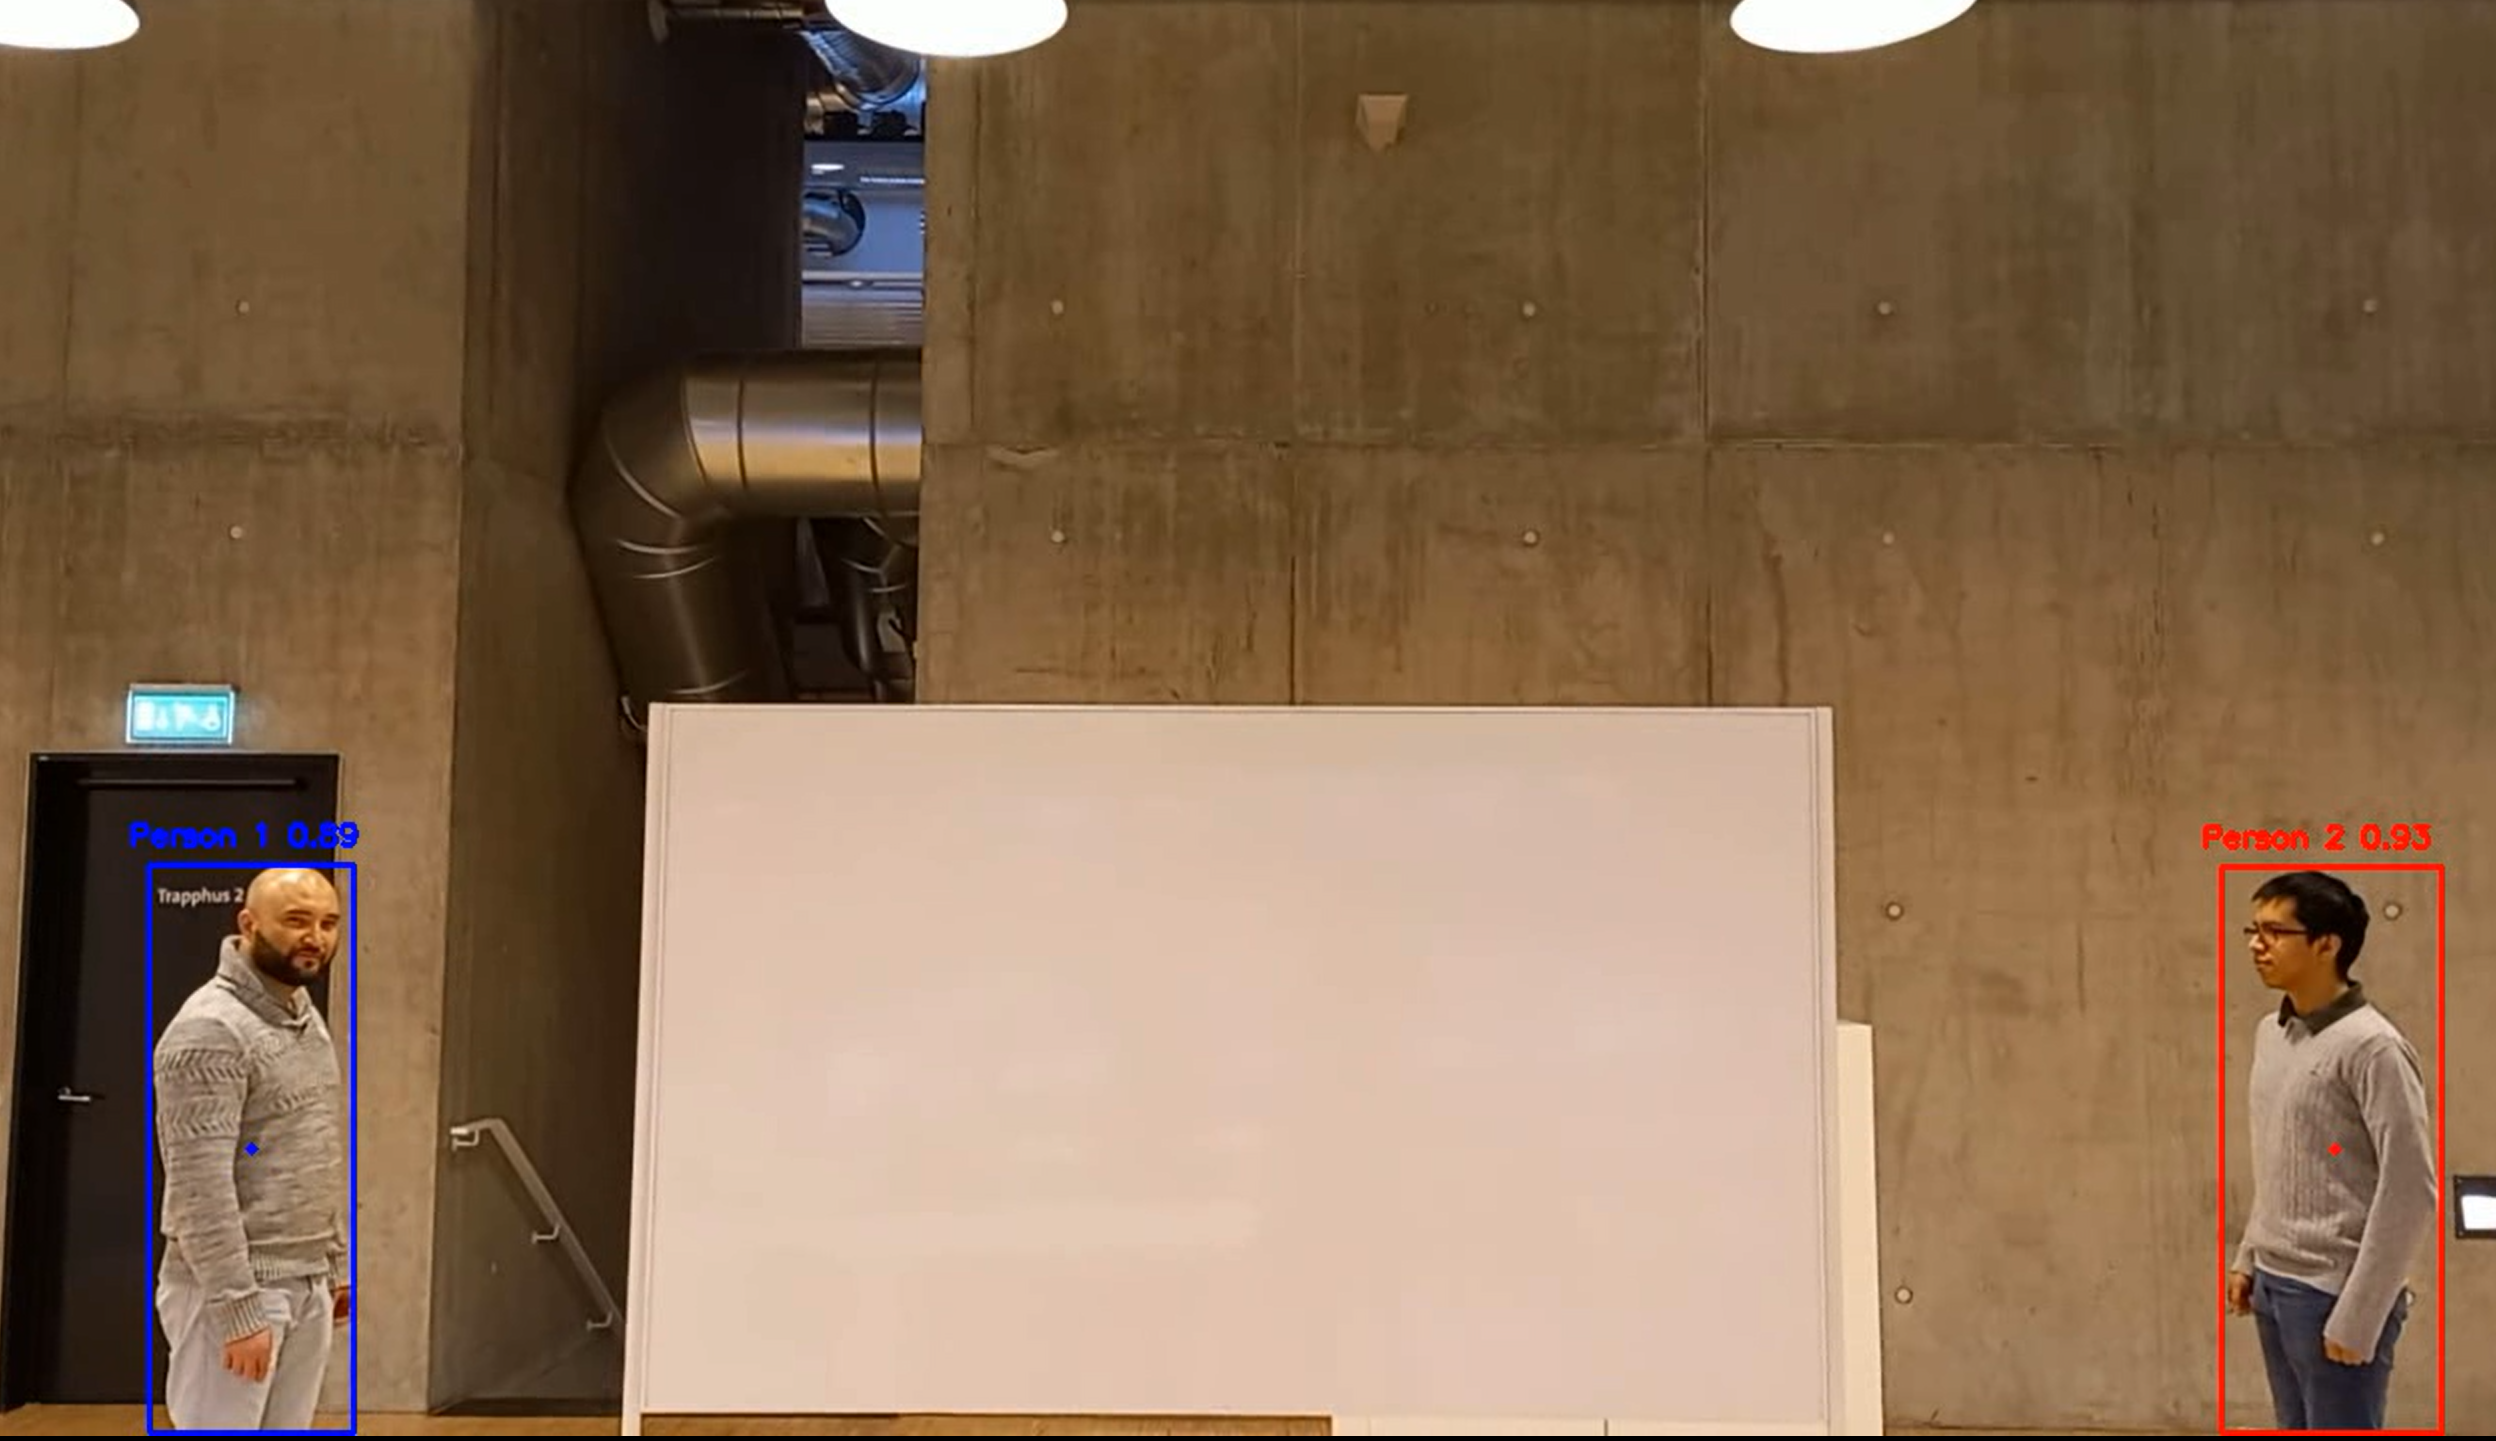
\includegraphics[width=0.5\linewidth]{two people passing whiteboard.png}
\caption{Two People When Passing Behind a Whiteboard}
\label{fig:two human passing}
\end{figure}

\subsubsection{Scenario: Two Individuals Crossing Paths}
Adopting the initial scenario's process noise parameters (\(std\_x = 0.000025\), \(std\_y = 0.0001\)), this test assumes a lower degree of motion unpredictability, the expectation is smooth and linear movements. The tracking system is evaluated for its capacity to accurately follow two individuals as they cross each other's paths, a situation that poses a high risk of track swapping or detection failures due to the proximity and potential for rapid, unanticipated changes in motion.

In instances of such crossings, the tracking algorithm faces considerable challenges. The primary issue lies in the system's limited ability to dynamically adapt to sudden alterations in direction or velocity. Consequently, the performance may be compromised, with notable errors. These inaccuracies are illustrated as either the incorrect continuation of tracks (leading to swapped identities) or missed detections altogether, particularly when the model's assumptions about motion continuity are violated by the movements characteristic of this scenario.

\begin{figure}[H]
\centering
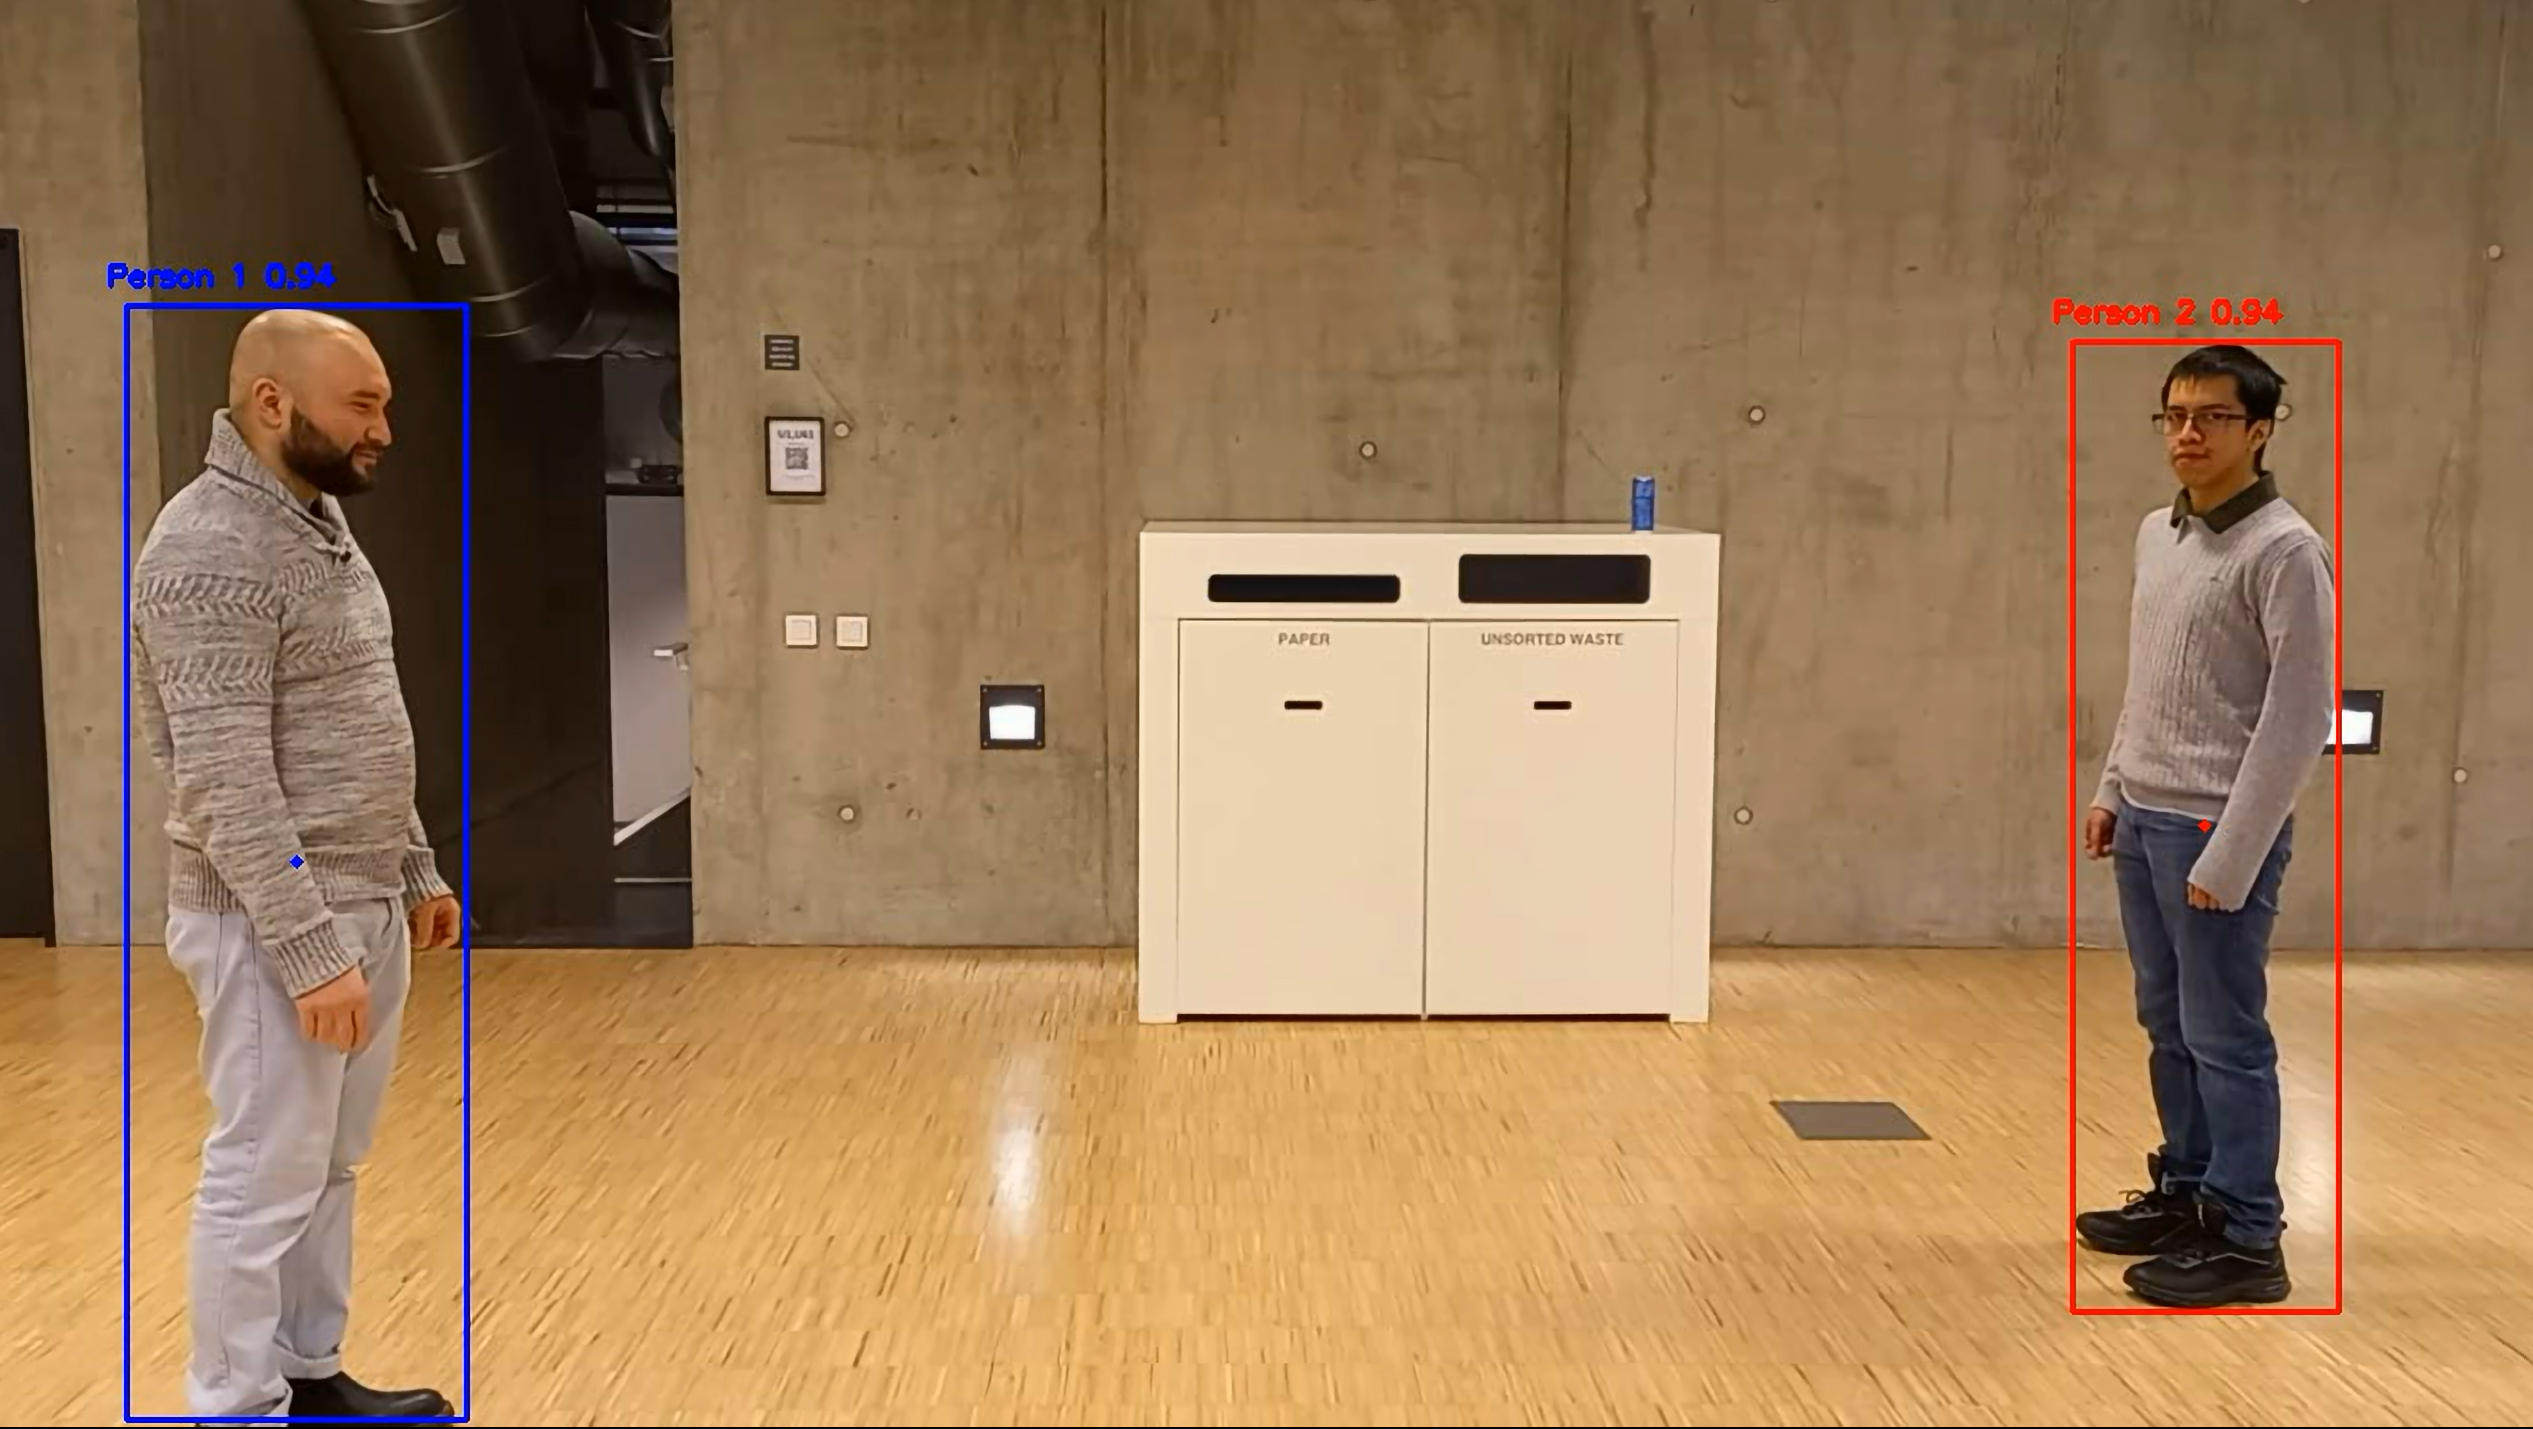
\includegraphics[width=0.5\linewidth]{two people passing.png}
\caption{Two People Passing Each Other}
\label{fig:two human}
\end{figure}

The video analyses provide good evidence of the tracking system's efficacy in managing scenarios where individuals cross paths, successfully avoiding potential track swaps or missed detections. This level of performance is largely attributable to the sophisticated detection capabilities of the YOLOv5 model, by combining it with an Extended Kalman Filter setup. The key to this success lies in the precise calibration of the process noise parameters (\(std\_x\) and \(std\_y\)), which are critical for accurately modeling the variance in motion observed in these dynamic interactions.

Moreover, the system's robust data association mechanism plays a pivotal role in ensuring that detections are consistently and accurately aligned with the correct tracks, even amidst the complexities of close proximity interactions between subjects. Such effectiveness in tracking accuracy, even in highly dynamic environments, highlights the system's potential applicability in real-world scenarios. These scenarios demand reliable tracking of multiple objects, which affirms the system's readiness for practical deployment and its contribution to advancing the field of computer vision-based tracking.

\section{Discussion}
\subsection{Implications of Bounding Box Dimension Variability}
Throughout this project, our tracking algorithms have relied on the dimensions and configurations of bounding boxes as indicators of subject movement and velocity. A notable challenge arises when an individual is only partially visible due to obstructions, leading to a reduction in the bounding box's size. This decrease is often misinterpreted by the algorithm as an indication of the subject either receding from the camera's view or decelerating. Such a change impacts the calculated center of the bounding box, which enforces the algorithm to recalibrate its predictions regarding the subject's precise location.

Particularly in situations where obstructions mask the lower portion of an individual's figure yet leave the central area unobscured, the algorithm may erroneously deduce alterations in the subject's velocity or trajectory. These inaccuracies are from the algorithm's dependence on bounding box dimensions to derive insights into movement patterns, which is a critical area for refinement in the pursuit of enhancing tracking precision.

\subsection{Degradation of Tracking Accuracy Due to Obstructions}

A factor affecting the efficacy of human tracking algorithms is the obstruction of the subject, resulting in partial or complete invisibility to the camera's lens. A prevalent presumption within these algorithms is the continuity of motion or the maintenance of constant acceleration by the subjects being tracked. However, this assumption becomes manifesting as tracking drift during instances of obstruction. In such scenarios, the algorithm persists in extrapolating the subject's trajectory based on previously observed motion patterns, disregarding the potential for sudden changes in behavior or direction that obstructions often induce. The reliance on outdated motion data under these circumstances can compromise the accuracy of subsequent position predictions, highlighting a crucial challenge in maintaining tracking reliability amidst visual interruptions.

\subsection{Error Measurement}

The error qualification in our project involves comparing the predicted locations of individuals tagged as "person" across a sequence of images against a set of predefined reference positions. For each frame, reference coordinates (\(x, y\)) are retrieved from a historical dataset. Subsequent detections classified as "person" are then identified, with their bounding box center points calculated. The Euclidean distance between the center of each detected bounding box and its corresponding reference coordinate is computed to serve as the metric of error, reflecting the precision of the prediction. Ignoring the initial measurement to avoid startup variance, these errors are depicted in a plot, showcasing the variation of error values through the frame sequence. This approach offers a clear visualization of positional discrepancies from the reference, which lights the detection system's accuracy over time.

\subsubsection{Error Analysis for a Single Individual Behind a Whiteboard}

Analyzing the error dynamics for a scenario where an individual moves behind a whiteboard reveals notable fluctuations in prediction accuracy over time. As illustrated in Figure \ref{fig:error one human}, the initial frames display a relatively consistent error rate, suggesting a stable prediction performance. However, increasing error magnitude is observed as the sequence progresses, with a spike occurring near the 150th frame. This increase aligns with the individual's movement behind the obstruction, as verified through video analysis. The observed trend of gradually increasing tracking error raises the challenges posed by occlusions in maintaining accurate positional predictions.

\begin{figure}[H]
\centering
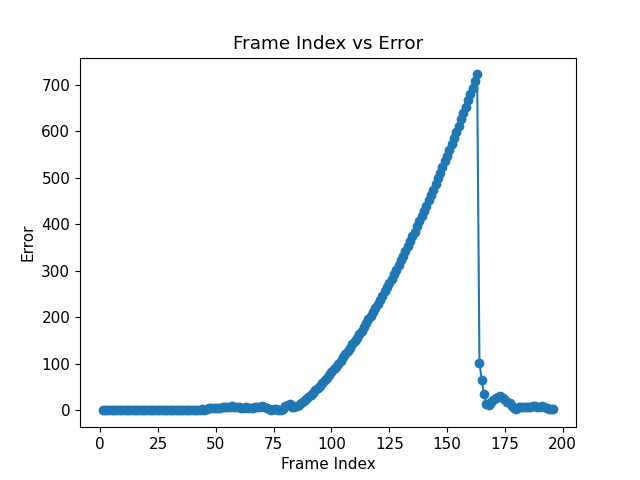
\includegraphics[width=0.5\linewidth]{plot_onepeople.png}
\caption{Frame Index vs Position Error}
\label{fig:error one human}
\end{figure}

The observed spike in prediction error around the 150th frame highlights a temporary decline in prediction accuracy, potentially attributable to sudden subject movements, occlusion, environmental changes, or specific limitations within the prediction algorithm. The subsequent rapid decrease in error suggests that the algorithm may possess corrective capabilities, allowing it to recover from transient inaccuracies.

Following this peak, the error rates settle at a marginally elevated level compared to the initial phase, implying a possible lasting effect of the disruption or an incremental drift in the algorithm's detection accuracy over time. The system's error rate stayed the same after the strange event, but it became less accurate. This means we need to carefully check how the system finds and predicts things. We need to figure out why the predictions are different and fix the problem so the system works better throughout the whole process.

\subsubsection{Error Dynamics for Two Individuals Behind a Whiteboard: Human 1}

The error associated with tracking Human 1 throughout the sequence shows considerable variation, characterized by multiple peaks and valleys. A notable spike in error is observed around the 40th frame, succeeded by a series of fluctuating error rates. These variations may reflect the challenges posed by sporadic occlusions or unpredictable movements, which complicate the tracking process. The frequent changes in error magnitude for Human 1 imply an enhanced sensitivity of the tracking system to this individual’s specific actions, or possibly, a more impact of whiteboard-induced occlusion on the prediction's fidelity. This pattern of increased error variability suggests the necessity for refining the tracking algorithm to better accommodate the dynamic nature of human movement and minimize the adverse effects of visual obstructions on prediction accuracy.

\begin{figure}[H]
\centering
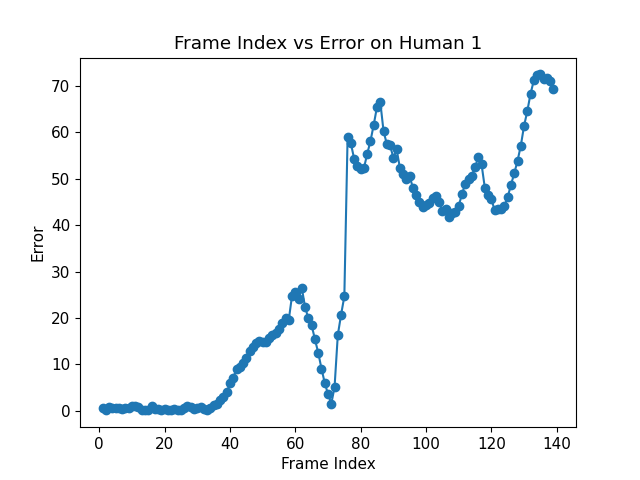
\includegraphics[width=0.5\linewidth]{plot_1.png}
\caption{Frame Index vs Position Error for Human 1}
\label{fig:two human behind board}
\end{figure}

\subsubsection{Error Analysis for Human 2 Behind a Whiteboard}

The error tracking for Human 2 starts low and stable, indicating effective tracking during the early frames. Around the 80th frame, however, there's a noticeable spike in error, likely due to Human 2 moving behind the whiteboard and becoming partially occluded. This moment of occlusion appears to disrupt the tracking accuracy significantly. Fortunately, the error quickly diminishes, suggesting that the system is able to adjust and regain accurate tracking once the subject is visible again. After when the spike rises, the error level rises slightly but then remains steady, indicating a minor, lasting impact of the occlusion event. This pattern suggests that while the tracking system is capable of recovering from disruptions caused by occlusion, there may be a slight, enduring adjustment in how it tracks the subject thereafter.

\begin{figure}[H]
\centering
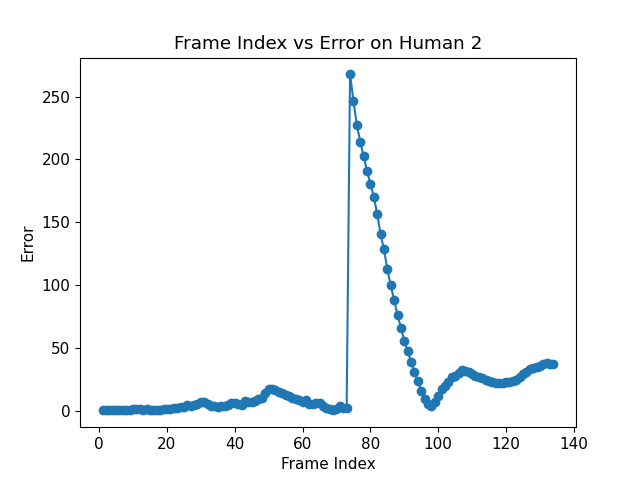
\includegraphics[width=0.5\linewidth]{plot_2.png}
\caption{Frame Index vs Position Error for Human 2}
\label{fig:human 2 behind board}
\end{figure}

\subsubsection{Comparative Error Analysis for Occlusion Events}

The error spikes observed in the tracking of both individuals highlight the disruptive impact of the whiteboard, suggesting moments where the tracking briefly loses accuracy. The variance in error behavior between the two subjects may depend on differences in their movement patterns, sizes, or how the tracking system responds to each. These discrepancies reveal the inherent difficulties of maintaining consistent tracking in environments where occlusions are present. The data from these plots clearly illustrate the importance of developing detection algorithms that are equipped to manage the complexities introduced by obstacles like the whiteboard, ensuring reliable tracking even in challenging conditions.

\subsubsection{Error Trends in Human 1 When Crossing Paths}

As shown in Figure \ref{fig:human1}, the error in tracking Human 1 starts low, indicating good tracking accuracy in the early frames. However, there's a sharp rise in error at around the 100th frame, which points to a possible brief drop in tracking precision. This spike could result from quick movements, someone blocking the view, or changes in the background that weren't anticipated.

After this spike, the error level begins to drop, suggesting that the tracking system is trying to correct itself and get back on track. Despite this effort, the error rate doesn't immediately smooth out but shows some ups and downs. This behavior indicates that the system is working to regain its initial accuracy but is still adjusting to the earlier disruption.

\begin{figure}[H]
\centering
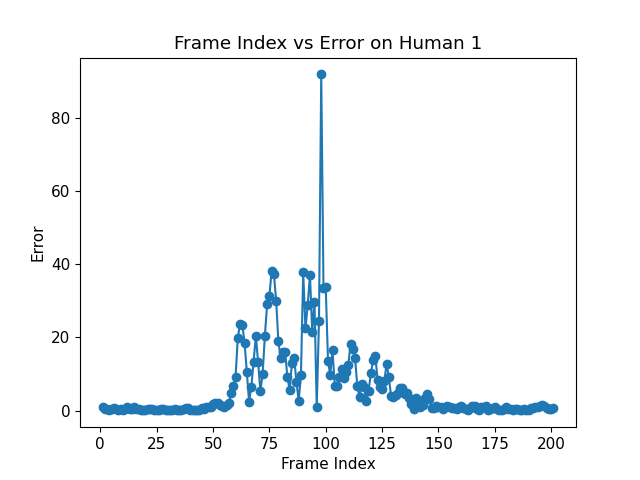
\includegraphics[width=0.5\textwidth]{plot_1_passing.png}
\caption{Frame Index vs Error on Human 1}
\label{fig:human1}
\end{figure}

\subsubsection{Error Analysis for Human 2 During Crossing Paths}

Figure \ref{fig:human2} shows the tracking error for Human 2, which is more uneven compared to Human 1. There are several high points in the error rate across the sequence. This suggests the tracking system faces ongoing issues while following Human 2. These challenges could come from sudden moves, people blocking the camera's view now and then, or the task of telling the two people apart. Unlike Human 1, the frequent error spikes for Human 2 indicate that the system is continually trying to adjust to these difficulties.

\begin{figure}[H]
\centering
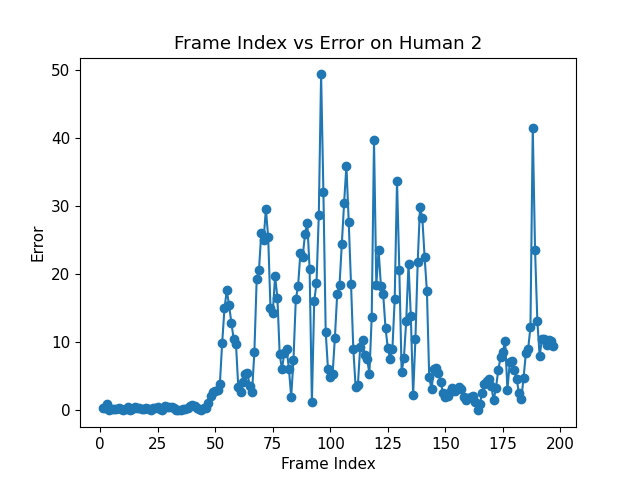
\includegraphics[width=0.5\textwidth]{plot_2_passing.png}
\caption{Frame Index vs Error on Human 2}
\label{fig:human2}
\end{figure}


\newpage

\subsection{Conclusion}

Combining YOLO for detecting objects and the Kalman Filter for predicting movement has shown great promise for tracking people in video surveillance. Our study shows that, despite its strong performance in many situations, issues like blockages and people moving close to each other can lead to notable mistakes in tracking.

The spikes in tracking errors, especially when people are hidden by something in the scene or when they walk close by each other, point out the challenges with tracking based on what the camera can see. The Kalman Filter does well with movements that don’t change much, but it struggles with sudden shifts in how fast or in what direction someone is going. Changes in how big or shaped the detected areas are can also make it harder to guess where someone is accurate, causing a gradual shift away from their true position.

Yet, the system often got back to tracking correctly after someone was no longer blocked from view. This suggests that making some adjustments, like tuning the noise settings better and getting better at matching data, could improve how it does in tricky situations. Looking ahead, we could try using smart learning methods to foresee blockages and tweak tracking as needed, along with better ways to tell apart people who are moving close to each other.

In conclusion, this project lays a solid groundwork for further developing automatic surveillance systems. With continuous progress in how computers can see and learn, we’re optimistic about solving these issues and reaching new heights in accurate and dependable human tracking.  

\bibliographystyle{alpha}
\bibliography{sample}

\end{document}